 
\begin{frame}[plain]{Wiring}{overview}
	Components:
	\center
	\pause
	\begin{itemize}
		\item Sensors
		\begin{itemize}
			\item Ultrasonic
			\item Camera
		\end{itemize}
		\pause
		\item Actuators
		\begin{itemize}
			\item Steering Servo
			\item Drive Motor
		\end{itemize}
		\pause
		\item Controll
		\begin{itemize}
			\item Nanoboard
			\item Raspberry Pi
		\end{itemize}
		\pause
		\item Power supply
		\begin{itemize}
			\item Battery
			\item H-Bridge
		\end{itemize}
	\end{itemize}
	
\end{frame}
 
 
 \begin{frame}[plain]{Wiring}{circuit layout}
	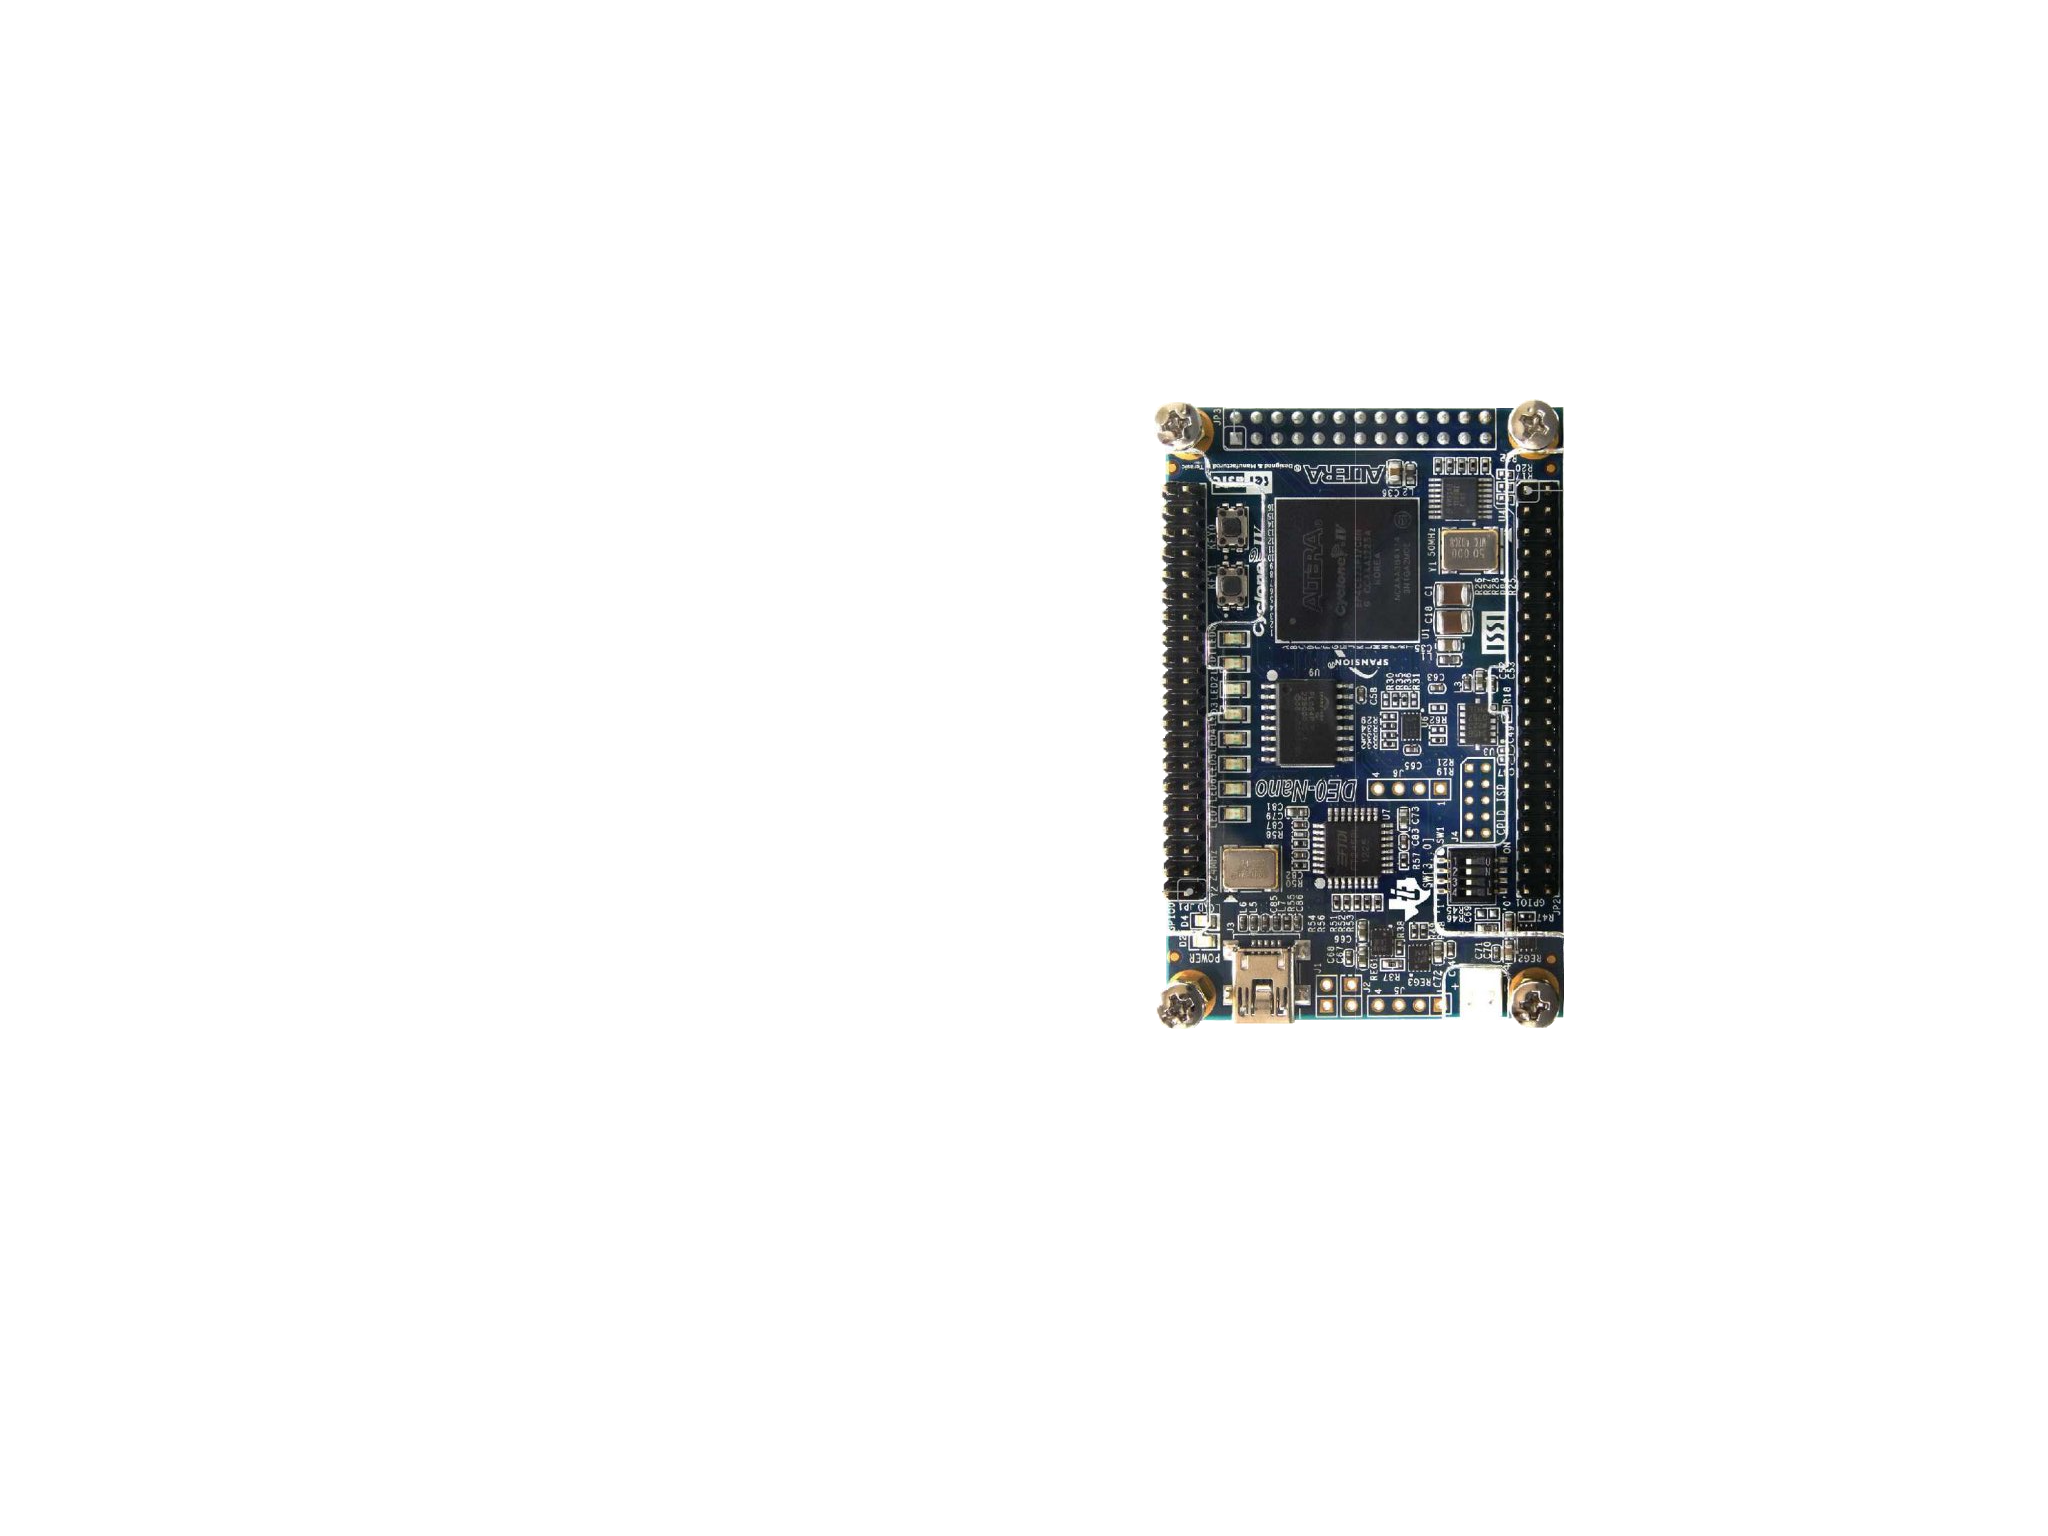
\includegraphics[width=\textwidth]{Feathergraphics/wiring1}
	\end{frame}
	
	
 \newcounter{ctra}
\setcounter{ctra}{2}
\whiledo {\value{ctra} < 13}%
{%
\begin{frame}[plain,noframenumbering]{Wiring}{circuit layout}
	\includegraphics[width=\textwidth]{Feathergraphics/wiring\the\value{ctra}}

\end{frame}
 \stepcounter {ctra}%
}
\addtocounter{page}{-16}